\mychapter{Background}{Background}{}\label{chap:background}

\section{Wastewater Treatment Works}
Municipal wastewater treatment plants purify our water using a series of steps. Large facilities typically rely on an effective biological method known as the activated sludge process. This system utilizes enormous tanks filled with beneficial microorganisms that naturally break down pollutants. During this process, the microorganisms convert the organic pollutants primarily into carbon dioxide, water, and new cellular biomass. These bacteria require a steady supply of oxygen to survive and work efficiently. To provide this air, facilities often use a technique called Fine Bubble Diffused Aeration (FBDA), which continuously pumps millions of tiny bubbles directly into the water. This happens in the \textbf{aerobic zones}. 

Once this active treatment is complete, the mixture flows into large circular settling tanks called \textbf{clarifiers}. The dense microbial biomass gradually settles to the bottom of the tank. This settling process leaves clear, treated water at the surface. Rather than discarding this settled biomass, the system continuously circulates it back to the initial tanks. Returning this activated sludge maintains a sufficient concentration of active microorganisms, ensuring the system can efficiently metabolize incoming organic matter.

Interestingly, someone who knows what to look for can tell a lot about how well these systems are performing just from aerial or satellite photos. A healthy FBDA unit churns the surface into a "leopard print" pattern, while a struggling one looks noticeably smoother. Clarifiers tell a similar story: when they are operating correctly, they separate out the solids and leave behind a clear liquid that looks black from above. When they are operating poorly, solids escape into the effluent and the surface turns green, cloudy, or uneven. Shown in Figure \ref{fig:treatment_comparison} are examples of functional and dysfunctional aerators and clarifiers, highlighting the visual cues that indicate their performance levels.

\begin{figure}[htbp]
    \centering 
    
    \begin{subfigure}[t]{0.31\textwidth}
        \centering
        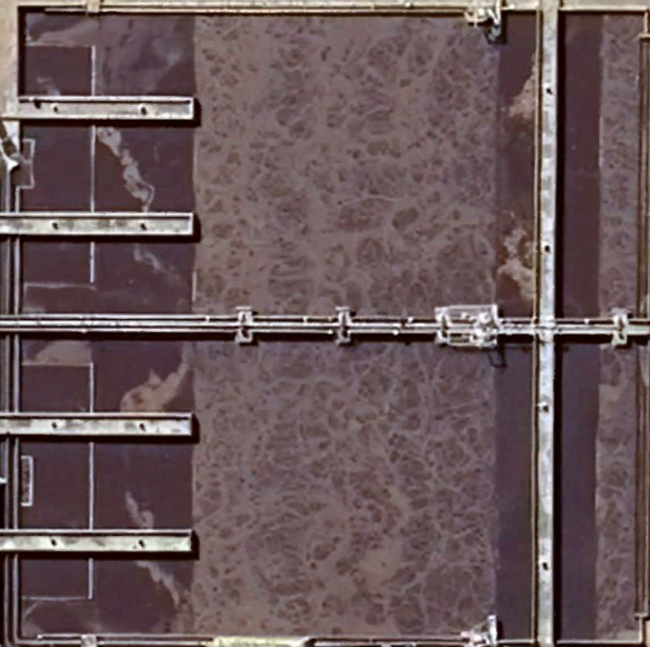
\includegraphics[width=\textwidth]{figures/aerobicfunc_background.png}
        \caption{Example of a functional aerator characterized by its "leopard print" pattern.}\label{fig:aerobic_func}
    \end{subfigure}
    \hfill
    \begin{subfigure}[t]{0.31\textwidth}
        \centering
        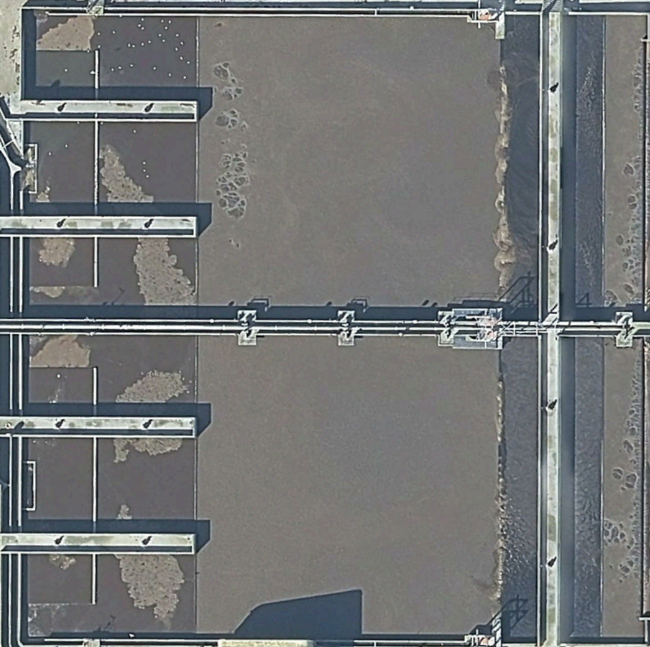
\includegraphics[width=\textwidth]{figures/aerobicdysfunc_background.png}
        \caption{Example of a dysfunctional aerator with a smooth surface, indicating poor performance.}\label{fig:aerobic_dysfunc}
    \end{subfigure}
    \hfill
    \begin{subfigure}[t]{0.31\textwidth}
        \centering
        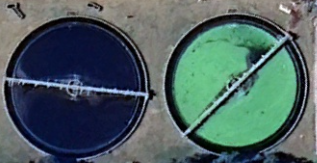
\includegraphics[width=\textwidth]{figures/clarifier_background.png}
        \caption{Functional clarifier on the left, dysfunctional clarifier on the right. The functional clarifier has a clear surface, while the dysfunctional one has solids floating on top.}\label{fig:clarifier}
    \end{subfigure}
    
    \caption{Visual comparison of functional and dysfunctional wastewater treatment components.}\label{fig:treatment_comparison}
\end{figure}
\section{Convolutional Neural Networks}
TODO

\section{Problem Statement}
Currently, the monitoring of wastewater treatment works (WWTW) is accomplished using on-site sensors, physical inspections, or the manual analysis of aerial photography by experienced personnel. While facilities equipped with sensors connected to automated control systems exist globally, they are currently not widely implemented in South Africa. Consequently, South African facilities rely primarily on on-site personnel to monitor operations. These personnel are required to sample the water at various stages of the treatment process at least once a day in an on-site laboratory, and at least once a month, samples should be sent to an independent laboratory for a complete analysis.

However, one or both of these testing protocols do not always occur. Incorrect measurements may be recorded, or tests may be omitted entirely. To detect such problems, physical site visits by officials are currently necessary. These physical inspections are expensive, time-consuming, and impractical to conduct with high frequency. Furthermore, on-site sensors, where utilized, are prone to failure and expensive to install and maintain.

The question this project aims to answer is whether a computer vision system can accurately identify the same visual indicators utilized by trained human operators (such as the characteristic surface turbulence of an aerator or the effluent clarity of a clarifier) to assess performance. A system evaluating satellite or aerial imagery could be utilized to detect problem cases. Specifically, a discrepancy between the reported laboratory data and the actual visual state observed in the imagery can be used to trigger corrective action. Ultimately, this study investigates the feasibility of leveraging historical satellite imagery to automatically monitor the functional state of Fine Bubble Diffused Aeration (FBDA) systems and clarifiers.


\section{Objectives}
To answer the above question, the project addresses the following three objectives:

\begin{enumerate}
    \item Prepare image datasets for experimentation and extract features by working with a set of labelled Google Earth satellite images taken on different dates to capture the visual states of WWTW components.
    \item Train classifiers to automatically determine the status of the aerobic zones(Functional, Suboptimal, Dysfunctional) and the Clarifiers(Functional, Dysfunctional, Scum, Empty), based on the image data.
    \item Evaluate the model's performance by testing it on a separate set of images and comparing its predictions to the known labels, using metrics like precision, recall, F1-score, Area under the ROC curve to quantify how well the model performs in classifying the different states of the WWTW components.
\end{enumerate}